\pdfbookmark{Общая характеристика работы}{characteristic}             % Закладка pdf
\section*{Общая характеристика работы}

\newcommand{\actuality}{\pdfbookmark[1]{Актуальность}{actuality}\underline{\textbf{\actualityTXT}}}
\newcommand{\progress}{\pdfbookmark[1]{Разработанность темы}{progress}\underline{\textbf{\progressTXT}}}
\newcommand{\aim}{\pdfbookmark[1]{Цели}{aim}\underline{{\textbf\aimTXT}}}
\newcommand{\tasks}{\pdfbookmark[1]{Задачи}{tasks}\underline{\textbf{\tasksTXT}}}
\newcommand{\aimtasks}{\pdfbookmark[1]{Цели и задачи}{aimtasks}\aimtasksTXT}
\newcommand{\novelty}{\pdfbookmark[1]{Научная новизна}{novelty}\underline{\textbf{\noveltyTXT}}}
\newcommand{\influence}{\pdfbookmark[1]{Практическая значимость}{influence}\underline{\textbf{\influenceTXT}}}
\newcommand{\methods}{\pdfbookmark[1]{Методология и методы исследования}{methods}\underline{\textbf{\methodsTXT}}}
\newcommand{\defpositions}{\pdfbookmark[1]{Положения, выносимые на защиту}{defpositions}\underline{\textbf{\defpositionsTXT}}}
\newcommand{\reliability}{\pdfbookmark[1]{Достоверность}{reliability}\underline{\textbf{\reliabilityTXT}}}
\newcommand{\probation}{\pdfbookmark[1]{Апробация}{probation}\underline{\textbf{\probationTXT}}}
\newcommand{\contribution}{\pdfbookmark[1]{Личный вклад}{contribution}\underline{\textbf{\contributionTXT}}}
\newcommand{\publications}{\pdfbookmark[1]{Публикации}{publications}\underline{\textbf{\publicationsTXT}}}

{\actuality} В последние десятилетия значительное внимание уделяется
экспериментам, направленным на поиск слабовзаимодействующих частиц,
чья природа выходит за рамки Стандартной модели. Как правило, такие
исследования требуют либо экстремальных энергий, либо накопления большой
статистики измерений в среднем энергетическом диапазоне. В последнем случае
широко применяются постановки с герметичным сбросом пучка, в которых
первичные частицы поглощаются массивной мишенью, а поиск редких событий
производится на основе большой статистики наблюдений, в котором решающее значение
играют точность реконструкции физических величин и надёжность оценки
фоновых процессов.

В то же время, средства автоматизации эксперимента,
во многом обеспечивающие требуемые точность и надёжность,
разрабатываются в условиях высокой динамики требований и
ограниченного жизненного цикла.
После завершения исследовательской программы они, как правило, утрачивают
актуальность как целостное решение, тогда как отдельные компоненты
могут представлять
ценность для повторного использования. Последнее обстоятельство
требует целенаправленной стратегии разработки программного обеспечения,
предполагающей повторное использование и интеграцию таких средств.
Руководящие ограничения такой стратегии опираются на ограниченный набор
особенностей, выбираемых на этапе проектирования информационных систем
с учётом специфики предметной области. Так например, использование триггерной
системы предполагает статистическую независимость физических
событий.

Объектом данного исследования является программное
обеспечения для реконструкции и анализа данных в физическом эксперименте.
В качестве предмета работы выступает создание
программного комплекса для реконструкции и анализа событий эксперимента
NA64\footnote{Эксперимент назван по внутренней номенклатуре CERN: <<North Area № 64>>}направленного
на поиск новых слабовзаимодействующих частиц,
%связывающих тёмный сектор с барионным веществом через портальные
%взаимодействия~\cite{NA64-first-paper},
из которых в работе рассматриваются
лёгкий аксион-подобный бозон~$a$~\cite{alps-PRD} и
т.н. тёмный фотон~$A'$~\cite{NA64-first-paper, DMG4-comphy-021}.

% степень проработанности
{\progress} В работах, посвящённых программному обеспечению для научных исследований
в целом %~\cite{software-for-science-CarverEtAl2016, lifecycle-lenhardt2014data}
и автоматизации физических экспериментов в частности %~\cite{Przedzinski2020PhD},
часто подчёркиваются отличия от промышленной разработки, требующие
глубокого погружения в предметную область и ограничивающее применимость
стандартных подходов к проектированию программного обеспечения, принятых в
индустрии. Несмотря на значительные усилия по созданию общих решений
и программных сред %~\cite{gaudi-framework-1, geant4-agostinelli, ROOT-framework, hep-roadmap-Albrecht2019},
специфика экспериментальной физики, связанная с
уникальностью экспериментальных постановок,
зачастую не позволяет полагаться на классические %централизованные
каскадные подходы.
В результате исследовательские группы реализуют решения, исходя
из текущих потребностей, действуя в рамках
гибких методологий разработки и формируя собственную программную базу
привязанную к локальным задачам. Экспертным сообществом отмечается,
что это нередко приводит к дублированию функциональности и затрудняет
долговременное сопровождение. %~\cite{elmer2018strategicplanscientificsoftware}.
В результате накопления технического долга перенос и внедрение
уже реализованных программ в новые
задачи оказывается зачастую менее оправданным, чем их повторная
реализация.
Тем не менее такой подход остаётся преобладающим и описывается
как общеупотребимая практика %<<ad hoc>> (или <<bottom-up>>~\cite{frameworks-Brun2011})
предполагающая индуктивный переход от ситуативных решений
к более общим системам.

{\aim} данной работы является разработка программного комплекса для
экспериментальной физики частиц обеспечивающего сопровождение
эксперимента на различных этапах его жизненного цикла, включая
моделирование, сопровождение набора данных, калибровку детекторов,
реконструкцию и анализ событий.
%в электромагнитных
%ливнях на основе параметрических моделей сигналов и ливней,
%а также аналитически управляемого моделирования фоновых/сигнальных
%процессов.

Для достижения поставленной цели, решаются следующие {\tasks}:
\begin{enumerate}[beginpenalty=10000]
    %\item Выделить типовые варианты использования  в рамках задач
    %автоматизации физического эксперимента.
    %\item Выделить архитектурные ограничения для программного комплекса,
    %обоснованные типовыми вариантами использования компьютерных
    %программ в рамках задач автоматизации физического эксперимента.
    \item Разработать спецификацию программной архитектуры,
    обеспечивающую основные задачи автоматизации физического эксперимента,
    в рамках архитектурных ограничений присущих экспериментам
    с логическим триггером.
    \item Реализовать архитектуру в виде
    обобщённых программ и алгоритмов, не подразумевающих специфику
    конкретного эксперимента и валидировать её посредством решения
    конкретных задач реконструкции и анализа событий NA64.
    \item Разработать и интегрировать в существующее специализированное
    программное окружение генератор событий для моделирования
    отклика установки на сигнальные события.
    \item Разработать и интегрировать систему генерации динамических
    машин состояния для выбора гипотез в задачах оптимизации, часто
    возникающих в рамках реконструкции физического события.
    \item Верифицировать предложенные реализации,
    применив к различным этапам жизненного цикла эксперимента,
    включающим Монте-Карло моделирование, сопровождение набора данных,
    калибровку детекторов, реконструкцию событий и анализ.
\end{enumerate}
При разработке и апробации программного комплекса необходимо
учесть, и, где это возможно, внедрять существующую алгоритмическую
базу.

{\methods}
С учётом сложившихся в науке практик создания компьютерных программ
прикладного уровня, целесообразно рассмотреть некоторые
подходы промышленной инженерии программного обеспечения,
учитывающие специфику предметной области и направленные
на инкрементную модель разработки. Таким требованиям вполне
отвечают т.н. гибкие (англ. \emph{agile})
методологии разработки, многие
из которых ставят приоритетом обеспечение высокой доступности
решений в рамках кратковременных циклов разработки.

На уровне конкретных технических средств, необходимо учесть
требования предъявляемые не только к длительности цикла разработки, но и
к быстродействию самих программ. Последнее условие значительно сужает
круг доступных выразительных средств, заставляя разработчиков
прибегать к сравнительно низкоуровневым решениям, в рамках которых
недостаток выразительности компенсируется за счёт высокой идиоматизации
(метапрограммирование, шаблоны, предметно-специфичные языки~\cite{perspectives-object-model-2012})
и инкапсуляции оптимизированных решений в рамках упрощённого
программного интерфейса.

Апробации реализованных технических решений осуществляются в рамках
конкретного эксперимента, чья постановка имеет глубокое методическое
обоснование. Она относится к семейству экспериментов с герметичным
сбросом пучка (англ. \emph{active beam-dump}). Методика измерений
включает поиск редких событий по сигнатуре недостающей энергии, а так
же регистрацию энерговыделения за массивным
поглотителем (англ. \emph{light shining through the wall}).
Статистическая интерпретация наблюдений формулируется
в рамках широко используемого в настоящее время метода CLs,
полно и непротиворечиво сформулированного в рамках частотной и байесовской
интерпретаций вероятности.

{\novelty}
\begin{enumerate}[beginpenalty=10000]
    \item Впервые для программных средств сопровождения
    физического эксперимента обосновано применение статического
    полиморфизма на основе объектных моделей
    %как базового механизма параметризации
    при синтезе программной архитектуры для последовательной
    обработки событий.
    \item Предложена эффективная алгоритмическая
    % вообще, алгоритмическая, но совет настаивает
    реализация генератора событий для симуляции
    рождения тёмного фотона в приближении спектра эквивалентных
    фотонов Вайцзеккера-Вильямса.
    %\item Разработана методика калибровки электромагнитного
    %калориметра не требующая полных априорных оценок
    %энерговыделения.
    %\item Подход, опирающийся на статический полиморфизм
    %специфичных для конкретного эксперимента объектных моделей
    %в качестве основного принципа выведения архитектуры применяется впервые.
    \item Впервые установлены верхние пределы на массу $m_a$ и константу
    смешивания $g_{a\gamma\gamma}$ в реакции $e^- + Z \to e^- + Z + a$
    для уровня статистической значимости $\alpha = 0{,}1$.
\end{enumerate}



%Разработана система автоматизации детектора КМД-2, включающая
%в себя комплекс программного обеспечения, предназначенного для
%выполнения следующих задач: чтения данных из электроники де-
%тектора; анализа данных в режиме реального времени и реализации
%на его основе третичного триггера и системы оперативного контроля
%качества данных; организации системы мониторинга детектора; организации
%системы управления детектором. Система автоматизации
%успешно проработала в течение всего срока эксплуатации детектора
%КМД-2.

{\defpositions}
\begin{enumerate}[beginpenalty=10000]
    % \item Разработано специализированное программное окружение для
    % решения ключевых задач реконструкции событий в экспериментах
    % физики высоких энергий, включая обработку данных трековых
    % детекторов и калориметров. Установлено соответствие архитектуры
    % данного окружения шаблону проектирования <<Конвейер>>~(Pipeline).
    \item Устройство модульного программного комплекса
    в парадигме обобщённого программирования
    для сопровождения полного
    цикла эксперимента по физике частиц,
    включая моделирование,
    накопление данных,
    калибровку детекторов,
    восстановление и анализ физических событий.
    %Комплекс реализован на основе статического полиморфизма,
    %в обобщённом виде и параметризуется ограниченным числом
    %параметров, специфичных для конкретного эксперимента
    %с триггерной системой, обеспечивая более короткие по сравнению
    %с существующими решениями циклы разработки.
    %По сравнению с существующими решениями обеспечивая
    %более короткие циклы разработки за счёт модульной структуры

    %\item Предложена эффективная алгоритмическая реализация генератора
    %событий для процессов фотообразования тёмной материи на основе
    %метода мажорирующих функций. Реализация интегрирована с моделями
    %генерации тёмных фотонов и лёгких аксионоподобных частиц.
    \item Эффективная алгоритмическая реализация генератора
    событий описывающего образование гипотетических
    частиц $A'$ (тёмный фотон) в реакциях рассеяния электронов
    на тяжёлых ядрах.
    
    \item Результат анализа экспериментальных данных NA64,
    соответствующих $2{,}84 \times 10^{11}$ электронов на мишени,
    %выполненный с использованием предложенных программных средств и методов,
    состоящий в том, что
    для реакции $e^{-} + Z \rightarrow e^{-} + Z + a$ 
    не обнаружено статистически значимого сигнала (при уровне значимости
    $\alpha = 0{,}1$) образования аксион-подобных частиц в
    диапазоне масс $m_a$ от~$10~\text{МэВ}$ до $100~\text{МэВ}$ и константы
    смешивания $g_{a \gamma \gamma}$ от~$2\times10^{-4}$ до~$10^{-2}$.
\end{enumerate}

{\contribution} Проектирование и реализация всех изложенных в работе
программ, за исключением описанных в
разделе <<Существующие программные решения>>, выполнены автором самостоятельно.

Алгоритмическая и программная реализация генератора~$A'$, лежащие в
основе \cite{DMG4-comphy-024, alps-PRD, DMG4-comphy-021}, выполнены
автором на основе существующих оценок сечения, в то время как внедрение и тестирование
генератора в интерфейсы окружения Geant4 выполнялись соавторами.

Обобщённая реализация алгоритма для поиска треков выполнена автором
на основе существующего описания алгоритма, с собственными дополнениями.
Тестирование и подстройка параметров выполнялись в сотрудничестве с
участниками коллаборации~NA64.

Автором предложен и реализованы метод реконструкции сигналов сэмплирующих
аналого-цифровых преобразователей
на основе подгонки функции отклика в конечной временной области и метод
калибровки электромагнитного калориметра.
Экспериментальная проверка алгоритма калибровки, настройка
алгоритма реконструкции сигналов, подбор параметров реконструкции трека
выполнялись в сотрудничестве с
участниками коллаборации~NA64.

Личный вклад автора в анализ данных ALP, опубликованный в \cite{alps-PRL}
состоит в статистическом обосновании критерия отбора фоновых событий,
моделировании и выделении исключённой области отсутствия сигнала на
основе анализа выполненного участниками коллаборации~NA64.

 % Характеристика работы по структуре во введении и в автореферате не отличается (ГОСТ Р 7.0.11, пункты 5.3.1 и 9.2.1), потому её загружаем из одного и того же внешнего файла, предварительно задав форму выделения некоторым параметрам

%Диссертационная работа была выполнена при поддержке грантов \dots

%\underline{\textbf{Объем и структура работы.}} Диссертация состоит из~введения,
%четырех глав, заключения и~приложения. Полный объем диссертации
%\textbf{ХХХ}~страниц текста с~\textbf{ХХ}~рисунками и~5~таблицами. Список
%литературы содержит \textbf{ХХX}~наименование.

\pdfbookmark{Содержание работы}{description}                          % Закладка pdf
\section*{Содержание работы}
Во \underline{\textbf{введении}} излагается актуальность
объекта исследований, проводимых в~рамках данной диссертационной работы,
%приводится обзор литературы по~изучаемой проблеме,
формулируется цель, ставятся задачи работы, излагается научная новизна
и практическая значимость представляемой работы.
%В~последующих главах
%сначала описывается общий принцип, позволяющий \dots, а~потом идёт
%апробация на частных примерах: \dots  и~\dots.


\underline{\textbf{Первая глава}} посвящена разработке
спецификаций, предложению и обоснованию архитектурных решений,
обеспечивающих варианты использования программного комплекса.

В разделе 1.1 описываются релевантные методологии разработки
программного обеспечения, излагаются основные требования к ним,
обосновываются черты гибридного подхода. Уточняется основная
терминология используемая в работе далее: виды полиморфизма,
точка расширения, архитектурные инварианты, использование
шаблонов C++ для реализации статического полиморфизма.
В соответствии с предложенной методологией в
разделе 1.2 фиксируется специфика предметной
области, включающую логический триггер и модель события,
а в разделе 1.3 кратко излагаются основные этапы жизненного
цикла эксперимента с точки зрения программного обеспечения,
включающие сценарии использования, сведённые в
иерархию, в основе которой лежат анализ, сопровождение набора данных
и процедуры калибровки детекторов. Подчёркивается
важность таких аспектов системы, как модульность,
детерминированность вычислений и изолированность компонент.
Аргументируется необходимость выведения модели события
и номенклатуры детекторов в точки расширения.
Раздел 1.4 завершает выведение основных архитектурных
ограничений и предлагает шаблоны
проектирования <<конвейер>>, <<издатель--подписчик>>
и <<фабрика>> в качестве механизма обеспечивающего
инвариантные свойства программного комплекса, а также
устанавливает основные качества коллекций в рамках
объектной модели события. Раздел 1.5 перечисляет существующие
программные решения --- общие окружения и инфраструктуры, а также
ряд популярных инструментов прикладного уровня.
Глава завершается разделом 1.6 содержащим итоговые
спецификации для организации программного комплекса.

% Вопрос №1: каким образом соотносится информация
%       о событии и его цифровая модель в смысле логического соответствия
%       статически-типизированным данным? (схемы, диаграммы, спецификации)

\underline{\textbf{Вторая глава}} посвящена описанию
эксперимента NA64 с целью получения предварительных численных
оценок и сведению обобщённых реализаций к конкретным программам
(инстанцированию шаблонов).
Раздел 2.1 описывает сигнальные процессы рождения $a$ и $A'$,
приводя лагранжиан взаимодействия, выражения для сечений и
распадной ширины. На основе приближения спектра эквивалентных
фотонов получены численные оценки для сигнального выхода
реакции $e^- + Z \rightarrow e^- + A' + Z$. В частности,
рассматривается сечение рождения $A'$:
\begin{comment}
%в соответствии с формулой \cite{bjorken}:
\[
\frac{1}{E^2_0} \frac{ d \sigma_{3 \rightarrow 2}}{d x d \cos{\theta_{A'}}} =
(8 \alpha \epsilon^2 \chi \beta_{A'}^2) \left[
    \frac{ 1 - x + x^2/2 }{U^2}
    + \frac{ (1-x)^2 m^2_{A'} }{U^4}
        \left( m^2_{A'} - \frac{U x}{1 - x} \right) \right],
\label{eq:bjorkenCS}
\]
где $x = E_0/E_{A'} \in (m_{A'}/E_0, 1 - m_{A'}/E_0)$ -- относительная энергия
$A'$, $\theta_{A'} \in [0, \pi]$ -- угол вылета, относительная скорость
$\beta = \sqrt{ 1 - m_{A'}/E_0 }$, и
$U = (E_0 \theta_{A'} )^2 x + m^2_{A'} (1-x)/x + m_e^2 x$.
Эффективный поток фотонов $\chi$ даётся интегральным выражением:
\begin{equation}
\chi = \int_{t_{min}}^{t_{max}} d t \frac{t - t_{min}}{t^2} G_2 (t),
\label{eq:photoFlux}
\end{equation}
где $G_2(t) = G_{2, el} + G_{2, inel}$ -- общий электромагнитный форм-фактор
\end{comment}
%в соответствии с формулой \cite{bjorken}:
\[
\frac{1}{E^2_0} \frac{ d \sigma_{2 \rightarrow 3}}{d x d \cos{\theta_{A'}}} \propto
\beta_{A'}^2 \left[
    \frac{ 1 - x + x^2/2 }{U^2}
    + \frac{ (1-x)^2 m^2_{A'} }{U^4}
        \left( m^2_{A'} - \frac{U x}{1 - x} \right) \right],
\label{eq:bjorkenCS}
\]
где $x = E_0/E_{A'}$ -- энергия $A'$ относительно энергии
налетающего лептона $E_0$,
$\theta_{A'}$ -- угол вылета,
$\beta = \sqrt{ 1 - m_{A'}/E_0 }$ и
$U = (E_0 \theta_{A'} )^2 x + m^2_{A'} (1-x)/x + m_e^2 x$.
Для дифференциального сечения такой формы вводятся следующие мажоранты:
\begin{equation*}
\begin{aligned}
    \mu_1(x, \theta) &= x^3 \theta \, 
        [E_0^2 \theta^2 x^2 + m_{A'}^2(1-x) + m_e^2 x^2]^{-2}, \\
    \mu_2(x) &= [2 E_0^2 \, (m_{A'}^2 (1 - x) + m_e^2 x ) ]^{-1},
\end{aligned}
\end{equation*}
используемые далее в методе обратной функции для построения
эффективного генератора псевдослучайных чисел с соответствующим
угловым и энергетическим распределением $A'$.
Приводятся оценки выхода сигнальных процессов для $A'$.
Описана аналогичная процедура для аксион-подобной частицы $a$.

Раздел 2.2 содержит краткое концептуальное описание
эксперимента NA64 и описывает общую номенклатуру
экспериментальных данных, имеющую значение для специализации обобщённых
реализаций программного комплекса.

Раздел 2.3 описывает основную номенклатуру
детекторов также являющуюся важным параметром в специализации
обобщённых реализаций. Приводятся описания основных
логических единиц триггерной системы: пучковых
счётчиков, калориметров и вето-детектора. Дано
краткое описание системы мечения первичных частиц,
организованной на основе магнитного спектрометра
и детектора синхротронного излучения. В перечне технических
параметров детектора особое значение имеет номенклатура
считывающей электроники, во многом определяющая
элементы объектной модели события.

Раздел 2.4 описывает сэмплирующие аналого-цифровые
преобразователи, применяемые для считывания сигналов
с фотоэлектронных умножителей и некоторых трековых
детекторов. Изложена проблема разрешения множественных
сигналов от близких по времени событий.

Раздел 2.5 содержит описание общей идеи метода CLs применяемого
для консервативной оценки чувствительности эксперимента.
В частности, на примере счётной статистики метод позволяет
строить исключённые области в пространстве
параметров сигнального процесса для заданного уровня
статистической значимости.

Глава завершается разделом 2.6 подводящим итоги главы
в виде описания функционального назначения элементов установки,
выделения общих и частных задач, соотносящихся с
систематизированными в предыдущей главе вариантами использования.

\underline{\textbf{Третья глава}} посвящена описанию реализации
программного комплекса и важным физическим результатам,
полученным с применением описанных в работе методов.

%картинку можно добавить так:
%\begin{figure}[ht]
%    \centerfloat{
%        \hfill
%        \subcaptionbox{\LaTeX}{%
%            
\includegraphics[scale=0.27]{latex}}
%        \hfill
%        \subcaptionbox{Knuth}{%
%            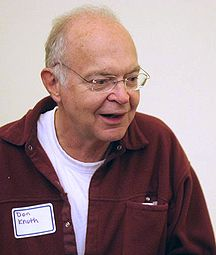
\includegraphics[width=0.25\linewidth]{knuth1}}
%        \hfill
%    }
%    \caption{Подпись к картинке.}\label{fig:latex}
%\end{figure}
%Формулы в строку без номера добавляются так:
%\[
%    \lambda_{T_s} = K_x\frac{d{x}}{d{T_s}}, \qquad
%    \lambda_{q_s} = K_x\frac{d{x}}{d{q_s}},
%\]
%\underline{\textbf{Вторая глава}} посвящена исследованию
%\underline{\textbf{Третья глава}} посвящена исследованию
%Можно сослаться на свои работы в автореферате. Для этого в файле
%\verb!Synopsis/setup.tex! необходимо присвоить положительное значение
%счётчику \verb!\setcounter{usefootcite}{1}!. В таком случае ссылки на
%работы других авторов будут подстрочными.
%Изложенные в третьей главе результаты опубликованы в~\cite{vakbib1, vakbib2}.
%Использование подстрочных ссылок внутри таблиц может вызывать проблемы.
%В \underline{\textbf{четвертой главе}} приведено описание

\FloatBarrier
\pdfbookmark{Заключение}{conclusion}                                  % Закладка pdf
В \underline{\textbf{заключении}} приведены основные результаты работы, которые заключаются в следующем:
%% Согласно ГОСТ Р 7.0.11-2011:
%% 5.3.3 В заключении диссертации излагают итоги выполненного исследования, рекомендации, перспективы дальнейшей разработки темы.
%% 9.2.3 В заключении автореферата диссертации излагают итоги данного исследования, рекомендации и перспективы дальнейшей разработки темы.

\begin{comment}
\begin{enumerate}
  \item На основе анализа \ldots
  \item Численные исследования показали, что \ldots
  \item Математическое моделирование показало \ldots
  \item Для выполнения поставленных задач был создан \ldots
\end{enumerate}
\end{comment}

% 5.3.3 В заключении излагают итоги выполненного исследования,
%     рекомендации, перспективы дальнейшей разработки темы
%
% На мой взгляд, можно было бы использовать термин «эксперимент с фиксированной мишенью» в качестве обобщающего для применения разработанного ПК, добавляя в необходимых для этого местах уточнение «например, для эксперимента NA64». Упоминание этих конкретных условий и объекта станет очень уместным в соответствующих разделах диссертации, например, в разделе о практической применимости и внедрении результатов. Более того, напоминаю, что в Заключении, кроме основных выводов должны быть представлены перспективы и предложения по использованию полученных результатов – CERN и коллаборация здесь вообще «не сыграют», а скорее навредят. В Заключении автореферата сейчас перечислены, в основном, частные достижения, а они там не нужны; придётся переформулировать в обобщающие научные выводы, исключив заодно всякие «коллаборации» и прочие «уникальные условия».

Разработана и обоснована архитектура программного комплекса
предназначенного для реконструкции и анализа событий в
рамках задач возникающих в физическом эксперименте с триггерной
системой.
Предложенная архитектура реализует ограниченный набор
архитектурных инвариантов:
модульность,
потоковая обработка,
наличие объектной модели события,
детерминированность и идемпотентность вычислений.
Сведение этих принципов в программную архитектуру и их
обобщённая реализация являются оригинальным техническим
решением, при помощи которого, в рамках рассмотренной гибридной методологии
разработки, в работе на конкретных
примерах обеспечен полный цикл сопровождения эксперимента -- показаны этапы
моделирования, реконструкции, анализа и обработки данных. В частности:
\begin{enumerate}
    \item Обобщённая реализация конвейера обработки данных обеспеченного
    калибровочной информацией и усиленного набором встраиваемых
    искусственных языков, позволяет проводить реконструкцию
    и анализ экспериментальных событий, включая этапы калибровки и
    мониторинга во время набора данных,
    \item Предложенный генератор модельных событий для процесса
    фотообразования частицы $A'$ (тёмный фотон) на основе аналитических
    сечений позволяет эффективно моделировать
    класс реакций образования гипотетических частиц на тяжёлых ядрах,
    связанных со Стандартной моделью электромагнитным взаимодействием,
    \item Предложенный метод калибровки герметичных детекторов не
    нуждается в априорных оценках энерговыделения, и позволяет проводить
    перекалибровку детектора во время набора данных,
    \item Реализованная подсистема генерации машин конечных состояний для
    решения задач минимизации и численной аппроксимации позволяет динамически
    обуславливать различные сценарии отбора гипотез. В частности, обобщённая
    реализация алгоритма отыскания треков позволяет снизить комбинаторный фон,
    а алгоритм подгонки функции отклика сигналов с сэмплирующих
    амплитудно-цифровых преобразователей позволяет восстанавливать сигналы
    с использованием конкурирующих гипотез априорной формы
    импульса (частично компенсируя ограничения на частоту Найквиста).
\end{enumerate}

Практическая значимость предложенных решений:

\begin{itemize}
    \item Архитектурные инварианты и реализованные механизмы
    расширения программного комплекса нацелены на разработку
    в рамках коротких циклов, допускают упрощенную интеграцию с
    другими экспериментами построенными на триггерной логике (включающие
    иные калориметрические конфигурации, трековые подсистемы,
    системы сбора данных), снижая затраты на сопровождение
    и повторное использование программного кода, и отвечая таким образом
    основным задачам автоматизации физического эксперимента.
    \item Параметрическая реконструкция сигналов и связанная с ней
    свёрточная модель ливня повышают устойчивость извлечения
    признаков (временные и амплитудные характеристики)
    при разных частотах дискретизации и геометриях
    сэмплирующих калориметров
    \item Генератор с аналитическими сечениями ускоряет
    численные оценки фона/сигналов в сценариях поиска слабых
    сигналов по сравнению с более общими методами, не
    учитывающими форму.
\end{itemize}


%а также явная спецификация точек расширения в
%рамках обобщённых шаблонных реализаций конвейера данных.
% нельзя ли как-то связать с "гибридной методологией разработки"?


\pdfbookmark{Литература}{bibliography}                                % Закладка pdf
При использовании пакета \verb!biblatex! список публикаций автора по теме
диссертации формируется в разделе <<\publications>>\ файла
\verb!common/characteristic.tex!  при помощи команды \verb!\nocite!

\ifdefmacro{\microtypesetup}{\microtypesetup{protrusion=false}}{} % не рекомендуется применять пакет микротипографики к автоматически генерируемому списку литературы
\urlstyle{rm}                               % ссылки URL обычным шрифтом
\ifnumequal{\value{bibliosel}}{0}{% Встроенная реализация с загрузкой файла через движок bibtex8
    \renewcommand{\bibname}{\large \bibtitleauthor}
    \nocite{*}
    \insertbiblioauthor           % Подключаем Bib-базы
    %\insertbiblioexternal   % !!! bibtex не умеет работать с несколькими библиографиями !!!
}{% Реализация пакетом biblatex через движок biber
    % Цитирования.
    %  * Порядок перечисления определяет порядок в библиографии (только внутри подраздела, если `\insertbiblioauthorgrouped`).
    %  * Если не соблюдать порядок "как для \printbibliography", нумерация в `\insertbiblioauthor` будет кривой.
    %  * Если цитировать каждый источник отдельной командой --- найти некоторые ошибки будет проще.
    %
    %% authorvak
    \nocite{vakbib1}%
    \nocite{vakbib2}%
    \nocite{vakbib3}%
    \nocite{vakbib4}%
    \nocite{vakbib5}%
    \nocite{vakbib6}%
    \nocite{vakbib7}%
    \nocite{vakbib8}%
    \nocite{vakbib9}%
    \nocite{vakbib10}%
    \nocite{vakbib11}%
    \nocite{vakbib12}%
    %
    %% authorwos
    \nocite{wosbib1}%
    %
    %% authorscopus
    \nocite{scbib1}%
    %
    %% authorpatent
    \nocite{patbib1}%
    %
    %% authorprogram
    \nocite{progbib1}%
    %
    %% authorconf
    \nocite{confbib1}%
    \nocite{confbib2}%
    %
    %% authorother
    \nocite{bib1}%
    \nocite{bib2}%

    \ifnumgreater{\value{usefootcite}}{0}{
        \begin{refcontext}[labelprefix={}]
            \ifnum \value{bibgrouped}>0
                \insertbiblioauthorgrouped    % Вывод всех работ автора, сгруппированных по источникам
            \else
                \insertbiblioauthor      % Вывод всех работ автора
            \fi
        \end{refcontext}
    }{
        \ifnum \totvalue{citeexternal}>0
            \begin{refcontext}[labelprefix=A]
                \ifnum \value{bibgrouped}>0
                    \insertbiblioauthorgrouped    % Вывод всех работ автора, сгруппированных по источникам
                \else
                    \insertbiblioauthor      % Вывод всех работ автора
                \fi
            \end{refcontext}
        \else
            \ifnum \value{bibgrouped}>0
                \insertbiblioauthorgrouped    % Вывод всех работ автора, сгруппированных по источникам
            \else
                \insertbiblioauthor      % Вывод всех работ автора
            \fi
        \fi
        %  \insertbiblioauthorimportant  % Вывод наиболее значимых работ автора (определяется в файле characteristic во второй section)
        \begin{refcontext}[labelprefix={}]
            \insertbiblioexternal            % Вывод списка литературы, на которую ссылались в тексте автореферата
        \end{refcontext}
        % Невидимый библиографический список для подсчёта количества внешних публикаций
        % Используется, чтобы убрать приставку "А" у работ автора, если в автореферате нет
        % цитирований внешних источников.
        \printbibliography[heading=nobibheading, section=0, env=countexternal, keyword=biblioexternal, resetnumbers=true]%
    }
}
\ifdefmacro{\microtypesetup}{\microtypesetup{protrusion=true}}{}
\urlstyle{tt}                               % возвращаем установки шрифта ссылок URL
